\chapter*{Proposition 7}
\label{prop:7}

\begin{figure*}[ht]
    \begin{center}
    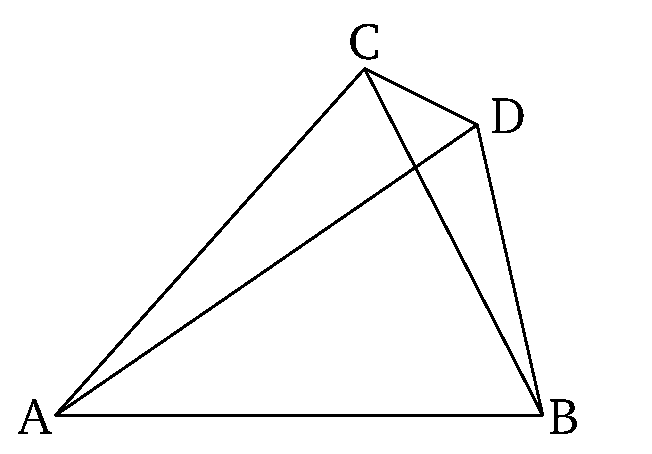
\includegraphics[width=0.5\linewidth]{figures/fig07e.eps}
    \label{fig:prop_7}
    \end{center}
\end{figure*}

On the same straight-line, two other straight-lines 
equal, respectively, to 
two (given) straight-lines (which meet) cannot be constructed (meeting)
at  a different point on the same
side (of the straight-line), but having the same ends as the given straight-lines.

For, if possible, let the two straight-lines $AC$, $CB$, equal to two other straight-lines $AD$, $DB$, respectively, have been constructed
on the same straight-line $AB$, meeting at different points, $C$ and $D$, on the
same side (of $AB$), and having the same ends (on $AB$). So $CA$ is equal to $DA$, having the same end $A$ as it, and $CB$ is equal to $DB$, having the
same end $B$ as it. And let $CD$ have been joined [Post.~\ref{post:1}].

Therefore, since $AC$ is equal to $AD$,  the angle $ACD$ is also equal to angle $ADC$ [Prop.~1.5].
Thus, $ADC$ (is) greater than $DCB$ [C.N.~\ref{cn:5}]. Thus, $CDB$ is much greater
than $DCB$ [C.N.~\ref{cn:5}]. Again, since  $CB$ is equal to $DB$, the angle $CDB$ is also equal to
angle $DCB$ [Prop.~1.5]. But it was shown that the former (angle) is also much
greater (than the latter). The very thing is impossible.

Thus, on the same straight-line, two other straight-lines equal, respectively, to  
two (given) straight-lines  (which meet) cannot be constructed (meeting)
at a different point on the same
side (of the straight-line), but having the same ends as the given straight-lines.
(Which is) the very thing it was required to show.


\section*{Commentary}

\begin{proposition}\label{proposition_7}\lean{Elements.Book1.proposition_7}\leanok
    $A$ and $B$ are two distinct points on a line $AB$. It is impossible to construct two distinct points $C$ and $D$ on the same side of $AB$, s.t., $|AC| = |AD|$ and $|CB| = |DB|$.
\end{proposition}
\begin{proof}
    \uses{proposition_5}\leanok
    Euclid's proof only works with the last two conditions, though he probably intended to prove a stronger version of Prop.~\ref{proposition_7} without these conditions, i.e., Prop.~\ref{proposition_7} below.
    To get there, we need to enumerate four possible cases (or two modulo permutations), whereas Euclid only considered the first one. 
    \begin{enumerate}
        \item[] $A$, $B$ are on the same of $CD$; $B$, $D$ are on the same side of $AC$: See Euclid's original proof.
        \item[] $A$, $B$ are on different sides of $CD$; $B$, $D$ are on the same side of $AC$: As Fig.~\ref{fig:prop_7'} shows, extend $AC$ to $E$ and $AD$ to $F$. Apply Prop.~\ref{proposition_5} to $\triangle ACD$ to derive $\angle~DCE = \angle~CDF$. Apply Prop.~\ref{proposition_5'} to $\triangle~BCD$ to derive $\angle~BCD = \angle~BDC$. Note that $\angle~DCE~>~\angle~BCD = \angle~BDC~>~\angle~CDF$. Contradiction. 
        \item[] $A$, $B$ are on the same side of $CD$; $B$, $D$ are on different sides of $AC$: Same as Euclid's proof, with $C$ and $D$ swapped.
        \item[] $A$, $B$ are on different sides of $CD$; $B$, $D$ are on different sides of $AC$: Same as Case 2, with $C$ and $D$ swapped.
    \end{enumerate}
\end{proof}


\begin{figure*}[ht]
    \begin{center}
    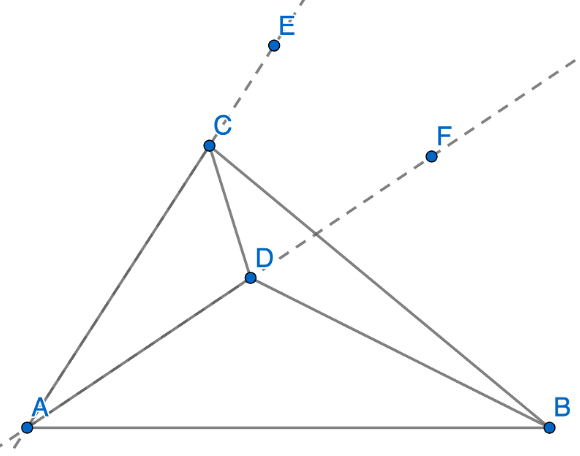
\includegraphics[width=0.5\linewidth]{figures/proposition_7'.png}
    \label{fig:prop_7'}
    \caption{$A$ and $B$ are on different sides of $CD$. $B$ and $D$ are on the same side of $AC$.}
    \end{center}
\end{figure*}

\begin{figure*}[ht]
    \begin{center}
    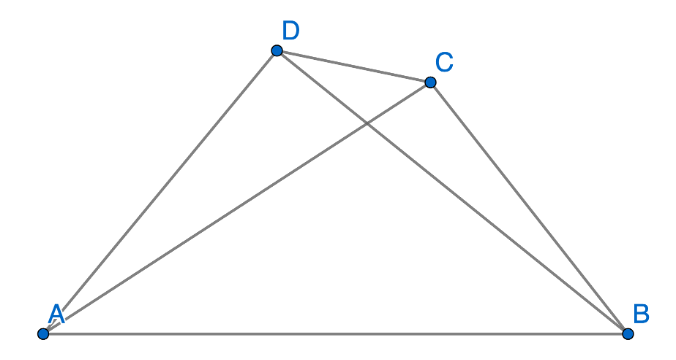
\includegraphics[width=0.5\linewidth]{figures/proposition_7''.png}
    \label{fig:prop_7''}
    \caption{$A$ and $B$ are on the same side of $CD$. $B$ and $D$ are on different sides of $AC$.}
    \end{center}
\end{figure*}

\begin{figure*}[ht]
    \begin{center}
    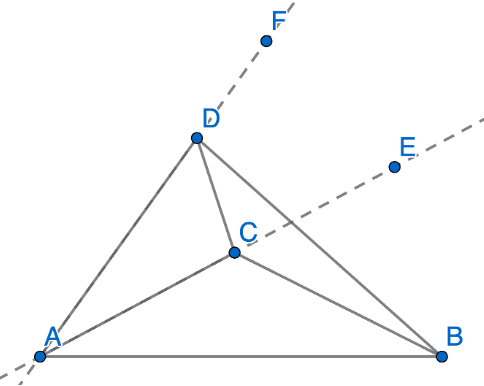
\includegraphics[width=0.5\linewidth]{figures/proposition_7'''.png}
    \label{fig:prop_7'''}
    \caption{$A$ and $B$ are on different sides of $CD$. $B$ and $D$ are on different sides of $AC$.}
    \end{center}
\end{figure*}
